\documentclass{standalone}
\usepackage{tikz}
\usetikzlibrary{patterns, positioning}

\begin{document}
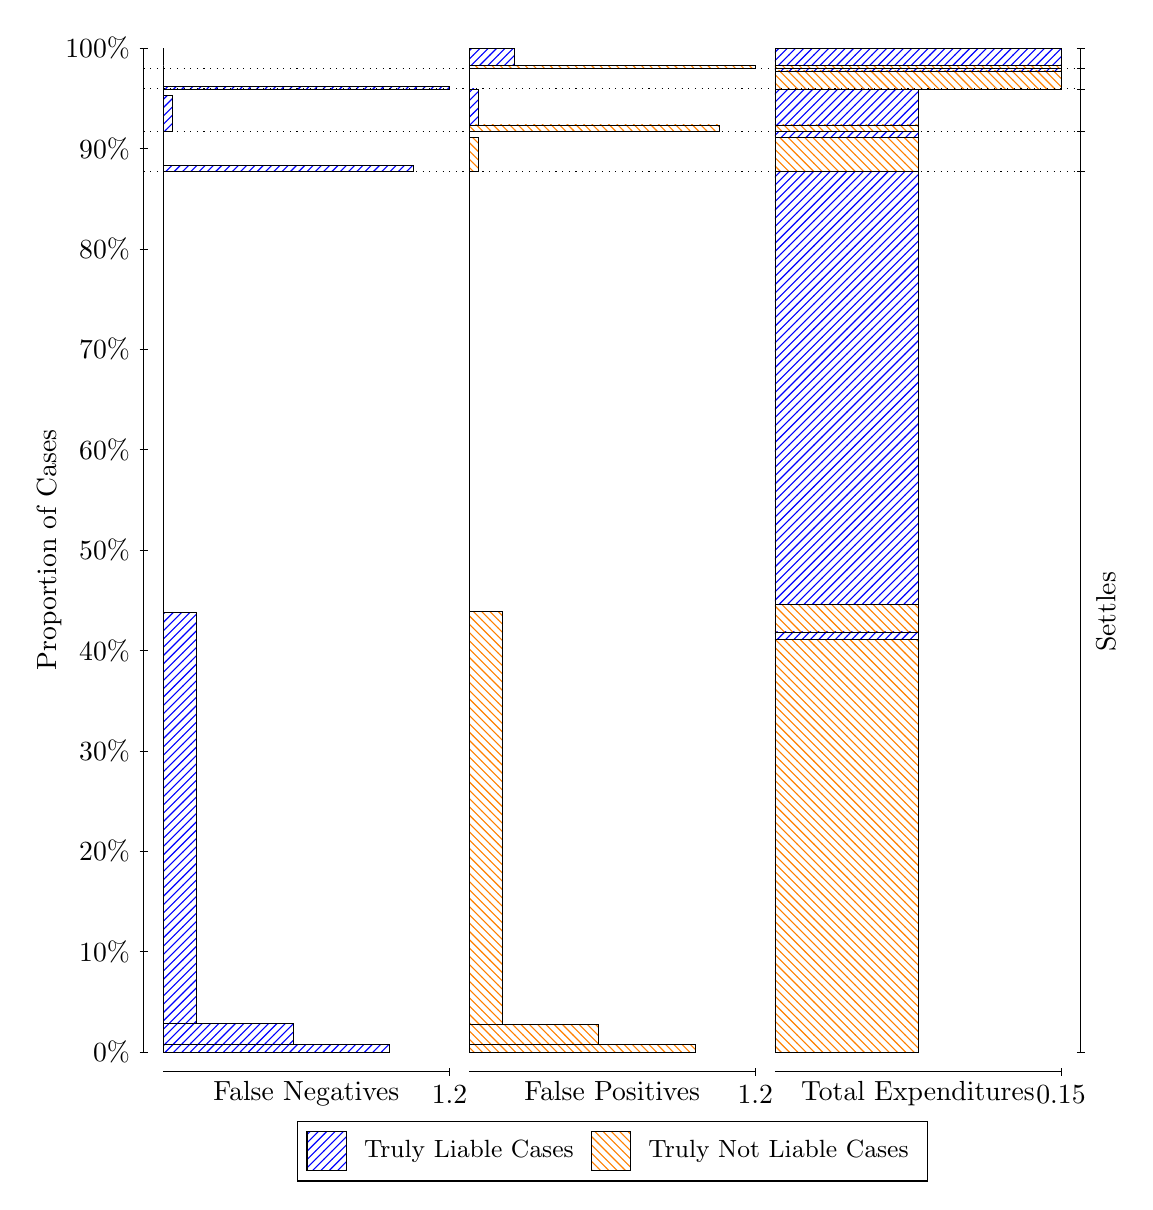
\begin{tikzpicture}
\draw[black, very thin] (1.5,1.75) -- (1.5,14.5);
\node[rotate=90, anchor=center] at (0.3, 8.125) {Proportion of Cases};
\draw[black, very thin] (1.45,1.75) -- (1.55,1.75);
\node[anchor=east] at (1.45, 1.75) {0\%};
\draw[black, very thin] (1.45,3.025) -- (1.55,3.025);
\node[anchor=east] at (1.45, 3.025) {10\%};
\draw[black, very thin] (1.45,4.3) -- (1.55,4.3);
\node[anchor=east] at (1.45, 4.3) {20\%};
\draw[black, very thin] (1.45,5.575) -- (1.55,5.575);
\node[anchor=east] at (1.45, 5.575) {30\%};
\draw[black, very thin] (1.45,6.85) -- (1.55,6.85);
\node[anchor=east] at (1.45, 6.85) {40\%};
\draw[black, very thin] (1.45,8.125) -- (1.55,8.125);
\node[anchor=east] at (1.45, 8.125) {50\%};
\draw[black, very thin] (1.45,9.4) -- (1.55,9.4);
\node[anchor=east] at (1.45, 9.4) {60\%};
\draw[black, very thin] (1.45,10.675) -- (1.55,10.675);
\node[anchor=east] at (1.45, 10.675) {70\%};
\draw[black, very thin] (1.45,11.95) -- (1.55,11.95);
\node[anchor=east] at (1.45, 11.95) {80\%};
\draw[black, very thin] (1.45,13.225) -- (1.55,13.225);
\node[anchor=east] at (1.45, 13.225) {90\%};
\draw[black, very thin] (1.45,14.5) -- (1.55,14.5);
\node[anchor=east] at (1.45, 14.5) {100\%};

\draw[black, very thin] (13.4,1.75) -- (13.4,14.5);
\draw[black, very thin] (13.35,1.75) -- (13.45,1.75);
\node[anchor=west] at (13.35, 1.75) {};
\draw[black, very thin] (13.35,12.929) -- (13.45,12.929);
\node[anchor=west] at (13.35, 12.929) {};
\draw[black, very thin] (13.35,13.444) -- (13.45,13.444);
\node[anchor=west] at (13.35, 13.444) {};
\draw[black, very thin] (13.35,13.981) -- (13.45,13.981);
\node[anchor=west] at (13.35, 13.981) {};
\draw[black, very thin] (13.35,14.245) -- (13.45,14.245);
\node[anchor=west] at (13.35, 14.245) {};
\draw[black, very thin] (13.35,14.5) -- (13.45,14.5);
\node[anchor=west] at (13.35, 14.5) {};

\draw[black, very thin, pattern color=blue, pattern=north east lines] (1.75,1.75) rectangle (4.6184,1.8462);
\draw[black, very thin, pattern color=blue, pattern=north east lines] (1.75,1.8462) rectangle (3.3946,2.1118);
\draw[black, very thin, pattern color=blue, pattern=north east lines] (1.75,2.1118) rectangle (2.1707,7.3365);
\draw[black, very thin, pattern color=orange, pattern=north west lines] (1.75,7.3365) rectangle (1.75,12.929);
\draw[black, very thin, pattern color=blue, pattern=north east lines] (1.75,12.929) rectangle (4.9244,13.005);
\draw[black, very thin, pattern color=orange, pattern=north west lines] (1.75,13.005) rectangle (1.75,13.444);
\draw[black, very thin, pattern color=blue, pattern=north east lines] (1.75,13.444) rectangle (1.8647,13.902);
\draw[black, very thin, pattern color=orange, pattern=north west lines] (1.75,13.902) rectangle (1.75,13.981);
\draw[black, very thin, pattern color=blue, pattern=north east lines] (1.75,13.981) rectangle (5.3833,14.016);
\draw[black, very thin, pattern color=orange, pattern=north west lines] (1.75,14.016) rectangle (1.75,14.245);
\draw[black, very thin, pattern color=orange, pattern=north west lines] (1.75,14.245) rectangle (1.75,14.28);
\draw[black, very thin, pattern color=blue, pattern=north east lines] (1.75,14.28) rectangle (1.75,14.5);
\draw[black, very thin, pattern color=orange, pattern=north west lines] (5.6333,1.75) rectangle (8.5018,1.8438);
\draw[black, very thin, pattern color=orange, pattern=north west lines] (5.6333,1.8438) rectangle (7.2779,2.1036);
\draw[black, very thin, pattern color=orange, pattern=north west lines] (5.6333,2.1036) rectangle (6.054,7.3422);
\draw[black, very thin, pattern color=blue, pattern=north east lines] (5.6333,7.3422) rectangle (5.6333,12.929);
\draw[black, very thin, pattern color=orange, pattern=north west lines] (5.6333,12.929) rectangle (5.7481,13.368);
\draw[black, very thin, pattern color=blue, pattern=north east lines] (5.6333,13.368) rectangle (5.6333,13.444);
\draw[black, very thin, pattern color=orange, pattern=north west lines] (5.6333,13.444) rectangle (8.8077,13.524);
\draw[black, very thin, pattern color=blue, pattern=north east lines] (5.6333,13.524) rectangle (5.7481,13.981);
\draw[black, very thin, pattern color=orange, pattern=north west lines] (5.6333,13.981) rectangle (5.6333,14.209);
\draw[black, very thin, pattern color=blue, pattern=north east lines] (5.6333,14.209) rectangle (5.6333,14.245);
\draw[black, very thin, pattern color=orange, pattern=north west lines] (5.6333,14.245) rectangle (9.2667,14.28);
\draw[black, very thin, pattern color=blue, pattern=north east lines] (5.6333,14.28) rectangle (6.207,14.5);
\draw[black, very thin, pattern color=orange, pattern=north west lines] (9.5167,1.75) rectangle (11.333,6.9886);
\draw[black, very thin, pattern color=blue, pattern=north east lines] (9.5167,6.9886) rectangle (11.333,7.0848);
\draw[black, very thin, pattern color=orange, pattern=north west lines] (9.5167,7.0848) rectangle (11.333,7.4384);
\draw[black, very thin, pattern color=blue, pattern=north east lines] (9.5167,7.4384) rectangle (11.333,12.929);
\draw[black, very thin, pattern color=orange, pattern=north west lines] (9.5167,12.929) rectangle (11.333,13.368);
\draw[black, very thin, pattern color=blue, pattern=north east lines] (9.5167,13.368) rectangle (11.333,13.444);
\draw[black, very thin, pattern color=orange, pattern=north west lines] (9.5167,13.444) rectangle (11.333,13.524);
\draw[black, very thin, pattern color=blue, pattern=north east lines] (9.5167,13.524) rectangle (11.333,13.981);
\draw[black, very thin, pattern color=orange, pattern=north west lines] (9.5167,13.981) rectangle (13.15,14.209);
\draw[black, very thin, pattern color=blue, pattern=north east lines] (9.5167,14.209) rectangle (13.15,14.245);
\draw[black, very thin, pattern color=orange, pattern=north west lines] (9.5167,14.245) rectangle (13.15,14.28);
\draw[black, very thin, pattern color=blue, pattern=north east lines] (9.5167,14.28) rectangle (13.15,14.5);
\draw[black, dotted] (1.5,12.929) -- (13.4,12.929);
\draw[black, dotted] (1.5,13.444) -- (13.4,13.444);
\draw[black, dotted] (1.5,13.981) -- (13.4,13.981);
\draw[black, dotted] (1.5,14.245) -- (13.4,14.245);
\draw[black, very thin] (1.75,1.5) -- (5.3833,1.5);
\node[anchor=north] at (3.5667, 1.5) {False Negatives};
\draw[black, very thin] (5.3833,1.45) -- (5.3833,1.55);
\node[anchor=north] at (5.3833, 1.45) {1.2};

\draw[black, very thin] (5.6333,1.5) -- (9.2667,1.5);
\node[anchor=north] at (7.45, 1.5) {False Positives};
\draw[black, very thin] (9.2667,1.45) -- (9.2667,1.55);
\node[anchor=north] at (9.2667, 1.45) {1.2};

\draw[black, very thin] (9.5167,1.5) -- (13.15,1.5);
\node[anchor=north] at (11.333, 1.5) {Total Expenditures};
\draw[black, very thin] (13.15,1.45) -- (13.15,1.55);
\node[anchor=north] at (13.15, 1.45) {0.15};

\node[black, centered, rotate=90] at (13.72, 7.3394) {Settles};





\draw (7.449999999999999,1.5) node[draw=none] (baseCoordinate) {};
\begin{scope}[align=center]
        \matrix[scale=0.5, draw=black, below=0.5cm of baseCoordinate, nodes={draw}, column sep=0.1cm]{
            \node[rectangle, draw, minimum width=0.5cm, minimum height=0.5cm, pattern=north east lines, pattern color=blue] {}; &
            \node[draw=none, font=\small] (B) {Truly Liable Cases}; &
            \node[rectangle, draw, minimum width=0.5cm, minimum height=0.5cm, pattern=north west lines, pattern color=orange] {}; &
            \node[draw=none, font=\small] (B) {Truly Not Liable Cases}; \\
            };
\end{scope}

\end{tikzpicture}
\end{document}